\cut{
1. (way ahead of time) train a statistical model over the training data
2. (at inference time) coarse-grain tokenization (i.e. finding Seqsets)
3a. run the statistical model over the user data, and use the (modified) 
    viterbi algorithm to find the most likely sequences
3b. populate histograms based on the most likely sequences
3c. select candidate histograms + structure, according to heuristics
3d. break down Seqsets using not just the most likely sequences
3e. recursively repeat, go to 3a.
4. apply rewriting involving blob finding to maximize the information 
   theoretic complexity score

We'll compose this algorithm by figure and explain it with running examples 
in Section 2.
}

\section{Description Inference Algorithm}\label{sec:algo}

We propose a multi-phase algorithm to attack the problem of
format inference for ad hoc data. The basic approach is to break the
input into units of repetition, called {\em chunks}, and then to
analyze these chunks for patterns that reveal the structure
of the data.  Depending upon the data source, the unit of repetition
might be a file, a collection of lines within a file that constitute
some notion of ``paragraph,'' a new-line terminated line, characters
terminated by pipes, \etc{}

The algorithm includes four main phases:
{\em training the statistical model}, 
{\em probablistically tokenizing} the raw data, 
performing recursive {\em structure discovery},
and using rewriting rules to do {\em format refinement}. 
This algorithm is similar to the one proposed in our earlier work
\cite{fisher+:dirttoshovels}.  
The new algorithm differs in that it defers decisions about
tokenization until structure discovery. 
In particular, the tokenization phase produces the set of {\em all
possible} token sequences for each data chunk in a data structure
called a \seqset{}.  The structure
discovery phase then incrementally selects the appropriate sequence from
the \seqset{} as it builds a description of the data.


%(3a) find the most probable token sequence for each chunk, and 
%     if that sequence of every chunk contains only 1 or 0 edges 
%     then return else go to (3b)
%(3b) construct histograms from the most probably sequences and 
%     predict a top-level structure;
%(3c) populate sub-components of the predicated structure with \seqset's
%     or sub-\seqset's;
%(3d) for each sub-component, recurse to (3a);

\begin{figure}[t]
\begin{centercode}
(1) Train a statistical model from labeled training data
(2) Tokenize raw data into \seqset{}s, one \seqset{} per chunk
(3) Discover initial structure using the \seqset{}s
(4) Apply rewriting rules to improve the overall structure
\end{centercode}
\caption{High-level Inference Algorithm}\label{fig:algo}
\end{figure}

\figref{fig:algo} summarizes the high-level algorithm.  In the
following sections, we explain the pieces in more detail using the
\texttt{yum.txt} format as a running example.
Because this algorithm shares the general structure of
the original algorithm, we only highlight the differences here, 
refering the reader to the earlier paper~\cite{fisher+:dirttoshovels}
for complete discussion of the original algorithm.

\subsection{Model training}

Before attempting to discover the structure of any particular format,
we train a statistical model to tokenize ad hoc data using a large
pool of sample data formats.  Intuitively, we can then use the
resulting model to infer formats for any ad hoc data source that uses
the tokens found in the training data.  Hence, we only need to
rerun this phase of the algorithm when given ad hoc data with
fundamentally different kinds of tokens.  

To train the statistical model, we label training data using a \pads{}
tool that takes a \pads{} description of a data source and labels each
atomic piece of data in the source with the \pads{} type used to parse
it.  By controlling the types in the supplied \pads{} description, we
control the set of tokens used to label the data.   Currently, we use
a set of tokens biased towards systems data, including
integer, float, time, date, ip address, hostname, file path, URL, 
word, id, white space and punctuation. 
%A given substring may be parsed by more than one of the token
%types, and we pick a token that best represent the meaning of the data.
We assume that parsing of tokens is {\em greedy}, \ie{},
each token matches the longest possible substring, hence
the string ``43.8'' can be parsed by sequences 
{\tt [int] [.] [int]}, {\tt [int] [.] [float]}, or {\tt [float]},
but not by {\tt [float] [.] [int]} or {\tt [float] [.] [float]},
because the token {\tt float} would parse the entire string, even though
the string ``43'' alone can be represented by a {\tt [float]}.

We have experimented with a number of different statistical models for
tokenization.  We defer a discussion of the particulars of these
models to \secref{sec:stats}.

\subsection{Probablistic tokenization}

When inferring a description, the algorithm computes the set of all
possible token sequences each data chunk.  Because these sequences
share subsequences, we organize them into a directed acyclic graph
called a \seqset{}. \figref{fig:seqset} shows the \seqset{} for the
substring ``2.2.13-4'' from a chunk in \figref{fig:yum}. It forms a
small part of the \seqset{} for the entire chunk.

\begin{figure}[th]
\begin{center}
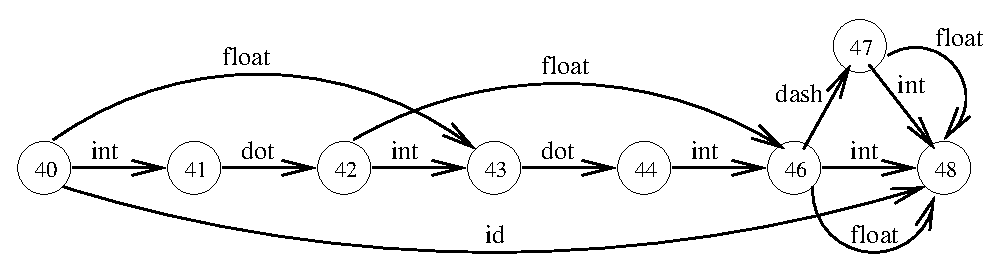
\epsfig{file=seqset.eps, width=0.9\columnwidth}
\end{center}
\caption{\seqset{} from parsing string ``2.2.13-4''}\label{fig:seqset}
\end{figure}
\noindent
Each edge in the \seqset{} represents an occurence of a token in the
data, while each vertex marks a location in the input.  If a token
edge ends at a vertex $v$, then $v$ indicates the position immediately
after the last character in the token.  The first vertex in a
\seqset{} marks the position before the first character in its
outgoing edges. 
The construction of the \seqset, though expensive, is done only once
per token training session.  The algorithm subsequently uses the
\seqset{} as input to the recursive structure discovery phase, which
updates the \seqset{} during each recursive call.

\begin{figure}[t]
\begin{centercode}
type description (* an intermediate representation *)
type seqset       (* a seqset *)
type seqsets = seqset list

(* A top-level description guess *)
datatype prophecy =
   BaseProphecy   of description
 | StructProphecy of seqsets list 
 | ArrayProphecy  of seqsets * seqsets * seqsets
 | UnionProphecy  of seqsets list

(* Guesses the best top-level description *)
fun oracle : seqsets -> prophecy

(* Implements a generic inference algorithm *)
fun discover (sqs:seqsets) : description =
 case (oracle sqs) of
   BaseProphecy b => b

 | StructProphecy sqss => 
     let Ts = map discover sqss in
     struct \{ Ts \}

 | ArrayProphecy (sqsfirst,sqsbody,sqslast) => 
     let Tfirst = discover sqsfirst in
     let Tbody  = discover sqsbody  in
     let Tlast  = discover sqslast  in
     struct \{ Tfirst; array \{ Tbody \}; Tlast; \}

 | UnionProphecy sqss => 
     let Ts = map discover sqss in
     union \{ Ts \}
\end{centercode}
\caption{A generic structure-discovery algorithm in Pseudo-ML.} 
\label{fig:structure-discovery}
\end{figure}

\subsection{Structure discovery}
The structure discover phase uses a {\em top-down}, {\em
divide-and-conquer} algorithm outlined in 
\figref{fig:structure-discovery} in the pseudo-ML function
\cd{discover}.  Each invocation of the \cd{discover} function
calls the \cd{oracle} function to guess the structure of the data represented
by the current set of \seqset{}s.  The oracle can prophecy
either a {\em base type}, a {\em struct}, an {\em array} or a {\em union}.
The {\tt oracle} function also partitions the input \seqset{}s into
sets of sub-\seqset{}s, each of which corresponds to a component in
the guessed structure.  The \cd{discover} function then recursively 
constructs the structure of each set of sub-\seqset{}s.

The {\tt oracle} function, which is the key to this magic does the
following. 

First, it runs the trained statistical model over the 
input \seqset's and assigns probabilities to all the edges of the \seqset's.
Next it computes the {\em most probable token sequence}, or MPTS, among all alternatives,
for each \seqset{} using a modified {\em Viterbi} algorithm \cite{rabiner89:hmm},
which will be discussed in detail in Section \ref{sec:stats}.
Then, based on the statistics of the tokens that appeared in the MPTSs,
it makes a predication about the structure of current set of
\seqset's, using the heuristics in \cite{fisher+:dirttoshovels}.
For example, during the first recursion, 
{\tt oracle} would predict that the top level structure of
a line in {\tt yum.txt} is 

\begin{centercode}
struct \{date;  ' '; time; ' '; word; ':'; ' '; id; TBD\}
\end{centercode}
which is a {\tt struct} containing 9 sub-structures and {\tt TBD} is a sub-structure
whose form is to be determined. At this point, the {\tt oracle} cuts
every \seqset{} in the input into 9 parts at the boundaries of the sub-structures,
i.e. at the vertices after tokens {\tt date}, {\tt space}, {\tt time}, etc. 
Sometimes, a cut at a particular location goes across existing edges of a
\seqset, then those edges are deemed irrelevant for next recurssion and removed.
For example, if we make a cut after the first {\tt float} token in the \seqset{}
in Fig. \ref{fig:seqset}, then the {\tt id}~ edge and the {\tt float} edge between
vertices 42 and 46 are removed, creating two new \seqset's in Fig. \ref{fig:cut}.

\begin{figure}[th]
\begin{center}
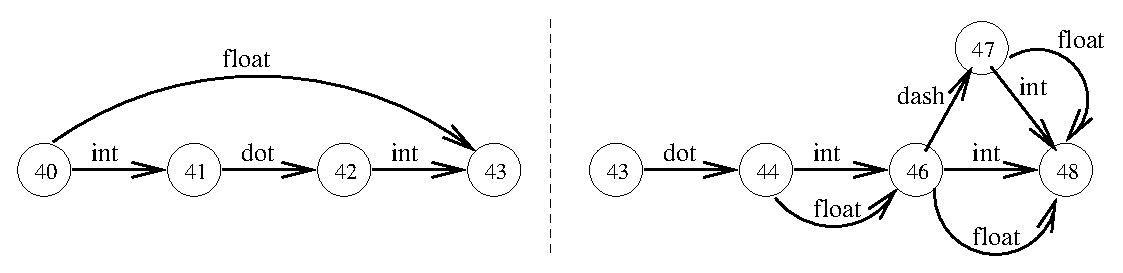
\epsfig{file=cut.eps, width=\columnwidth}
\end{center}
\caption{Cutting \seqset{} for ``2.2.13-4'' after the first float token} \label{fig:cut}
\end{figure}

Finally, the {\tt oracle} function returns the predicated structure as a ``prophecy''
along with the cut up \seqset's. 

\subsection{Format refinement with blob-finding}
The refinement phase follows the structure discovery phase to
improve the initial rough structure by applying a series of
rewriting rules. Here a new ``blob-finding'' rule is added to
the original algorithm. The purpose of this rule is to identify
``message-like'' structures in the intermediate structure and rewrite them into
a single token called {\em blob}, and thus reduce the overall complexity
of the description and increase readability. The blob-finding rule is applied
from bottom up and converts each sub-structure that is
determined to be overly complex and has a terminating pattern into a
blob. The \pads{} parser needs the terminating pattern to
know where the blob ends. Adjacent blobs are merged together. 

To determine whether a given structure is a blob, 
we compute a parameter called {\em variance} for the structure. 
It measures the total number of union/switch/enum
branches and different array lengths in the given 
structure. When the ratio between the variance and the amount of the data
this structure represents exceeds a threshold, the structure is
determined to be a possible blob. 
